\documentclass[12pt]{article}

\usepackage{graphics}
\usepackage{amsmath}
\usepackage{amsfonts}
\usepackage{amssymb}
\usepackage{blkarray}
\newcommand{\matindex}[1]{\mbox{\scriptsize#1}}
\usepackage[table]{xcolor}
\newcommand\scalemath[2]{\scalebox{#1}{\mbox{\ensuremath{\displaystyle #2}}}}



%\usepackage[active]{srcltx} % SRC Specials for DVI Searching

% Over-full v-boxes on even pages are due to the \v{c} in author's name
\vfuzz2pt % Don't report over-full v-boxes if over-edge is small

% THEOREM Environments ---------------------------------------------------

 \newtheorem{thm}{Theorem}[section]
 \newtheorem{cor}[thm]{Corollary}
 \newtheorem{lem}[thm]{Lemma}
 \newtheorem{prop}[thm]{Proposition}
 %\theoremstyle{definition}
 \newtheorem{defn}[thm]{Definition}
 %\theoremstyle{remark}
 \newtheorem{rem}[thm]{Remark}
 \numberwithin{equation}{section}
% MATH -------------------------------------------------------------------
 \DeclareMathOperator{\RE}{Re}
 \DeclareMathOperator{\IM}{Im}
 \DeclareMathOperator{\ess}{ess}
 \newcommand{\eps}{\varepsilon}
 \newcommand{\To}{\longrightarrow}
 \newcommand{\h}{\mathcal{H}}
 \newcommand{\s}{\mathcal{S}}
 \newcommand{\A}{\mathcal{A}}
 \newcommand{\J}{\mathcal{J}}
 \newcommand{\M}{\mathcal{M}}
 \newcommand{\W}{\mathcal{W}}
 \newcommand{\X}{\mathcal{X}}
 \newcommand{\BOP}{\mathbf{B}}
 \newcommand{\BH}{\mathbf{B}(\mathcal{H})}
 \newcommand{\KH}{\mathcal{K}(\mathcal{H})}
 \newcommand{\Real}{\mathbb{R}}
 \newcommand{\Complex}{\mathbb{C}}
 \newcommand{\Field}{\mathbb{F}}
 \newcommand{\RPlus}{\Real^{+}}
 \newcommand{\Polar}{\mathcal{P}_{\s}}
 \newcommand{\Poly}{\mathcal{P}(E)}
 \newcommand{\EssD}{\mathcal{D}}
 \newcommand{\Lom}{\mathcal{L}}
 \newcommand{\States}{\mathcal{T}}
 \newcommand{\abs}[1]{\left\vert#1\right\vert}
 \newcommand{\set}[1]{\left\{#1\right\}}
 \newcommand{\seq}[1]{\left<#1\right>}
 \newcommand{\norm}[1]{\left\Vert#1\right\Vert}
 \newcommand{\essnorm}[1]{\norm{#1}_{\ess}}
\usepackage{graphicx}
\usepackage{amsmath}
\usepackage{amsfonts}
\usepackage{amssymb}
%TCIDATA{OutputFilter=latex2.dll}
%TCIDATA{CSTFile=LaTeX article (bright).cst}
%TCIDATA{Created=Fri Nov 02 10:44:42 2001}
%TCIDATA{LastRevised=Mon Dec 10 11:56:49 2001}
%TCIDATA{<META NAME="GraphicsSave" CONTENT="32">}
%TCIDATA{<META NAME="DocumentShell" CONTENT="General\Blank Document">}
%TCIDATA{Language=American English}
\newtheorem{theorem}{Theorem}
\newtheorem{acknowledgment}[theorem]{Acknowledgment}
\newtheorem{algorithm}[theorem]{Algorithm}
\newtheorem{axiom}[theorem]{Axiom}
\newtheorem{case}[theorem]{Case}
\newtheorem{claim}[theorem]{Claim}
\newtheorem{conclusion}[theorem]{Conclusion}
\newtheorem{condition}[theorem]{Condition}
\newtheorem{conjecture}[theorem]{Conjecture}
\newtheorem{corollary}[theorem]{Corollary}
\newtheorem{criterion}[theorem]{Criterion}
\newtheorem{definition}[theorem]{Definition}
\newtheorem{example}[theorem]{Example}
\newtheorem{exercise}[theorem]{Exercise}
\newtheorem{lemma}[theorem]{Lemma}
\newtheorem{notation}[theorem]{Notation}
\newtheorem{problem}[theorem]{Problem}
\newtheorem{proposition}[theorem]{Proposition}
\newtheorem{remark}[theorem]{Remark}
\newtheorem{solution}[theorem]{Solution}
\newtheorem{summary}[theorem]{Summary}
\newenvironment{proof}[1][Proof]{\textbf{#1.} }{\ \rule{0.5em}{0.5em}}
\renewcommand\refname{}
\renewcommand\thefootnote{}
\textheight=9in \topmargin=-0.6in \everymath{\displaystyle}
\textwidth=6.5in \oddsidemargin=0.05in
\renewcommand\arraystretch{1.5}
\newenvironment{amatrix}[1]{%
  \left[\begin{array}{@{}*{#1}{c}|c@{}}
}{%
  \end{array}\right]
}
\includeonly{}
\usepackage{amsfonts}
\usepackage{amssymb}
\usepackage{eucal}
\usepackage{multicol}
\usepackage[c]{mcode}
\usepackage{listings}
\everymath{\displaystyle}
\graphicspath{{C:/Users/michael/Documents/Graduate School/Stochastic Processes and Modeling/}}

\begin{document}

{\large\bf MATH 6600, Homework 4, 12-16-2015}

\vspace{6 ex}

{\bf Name: Michael Hennessey} \hfill

\vspace{6 ex}

\begin{section}{Calculation and Modeling Problems}
\begin{subsection}{Continuous Time Machine Repair Model}
Herein we model a simple assembly line made of $N$ of the same type of machines, all available for service. However, only $M$ machines can be in use at any given time. Each machine has a rate $\mu_{\text{on}}$ of failing while operating, and $\mu_{\text{off}}$ of failing while dormant. We assume that the probability a machine fails in a given interval is independent of its history and of the status of other machines. Broken machines are sent to a service facility, which can handle a maximum of $R$ machines at a time. The repair time for a machine under service is an exponentially distributed random variable with average $T_r$.
\begin{enumerate}
    \item Construct a continuous-time Markov chain model for the state of the system of machines.\\

    Solution:\\

    Let $X(t)$ be the number of working machines, either in use or dormant. Clearly, $X(t)$ is a finite state birth and death chain using the assumptions in the set up of the model above. Then the number in use is $\min\{X(t),M\}$ and the number of dormant machines is $\max\{0,X(t)-M\}$. If we then let $Y(t)=N-X(t)$ be the number of broken machines we can similarly define the number of machines in repair and the number of machines waiting for repair. The number of machines in repair is $\min\{Y(t),R\}$ and the number waiting for repair is $\max\{0,Y(t)-R\}.$ We use these definitions, because once $X(t)$ is known, we can use it to define any of the other quantities needed.\\
    Thus we define the transition rates of the birth and death process:
    the birth rate is as follows
    $$\lambda_n=T_r\min\{N-n,R\}=\left\{\begin{array}{cc}T_r R,&n=0,1,...,N-R\\T_r(N-n),&n=N-R+1,...,N-1\end{array}\right..$$
    This is derived from the fact that the birth rate must be exponentially distributed with mean $T_r$ and that a maximum of $R$ machines can be repaired simultaneously. Similarly, the death rate is
    $$\mu_n=\left\{\begin{array}{cc}\mu_\text{on} n,&n=1,...,M\\ \mu_\text{on}+\mu_\text{off}(n-M),&n=M+1,...,N\end{array}\right..$$
    The death rate is derived similarly using the rates $\mu_\text{on}$ and $\mu_\text{off}$ along with the constraints on how many machines can be in use at any time.\\
    Here we note, for simplicity, that we assume travel time and the time a machine takes to be replaced has been factored into the calculation of the repair rate. Thus we are ready to write the transition rate matrix $A$.
    \[\scalemath{0.55}{A=\left[\begin{array}{ccccccc}
    -T_r R&T_r R\\
    \mu_\text{on}&-(T_r R+\mu_\text{on})&T_r R\\
    &2\mu_\text{on}&-(2\mu_\text{on}+T_r R)&T_r R\\
    \\
    &&(N-R+1)\mu_\text{on}&-((N-R+1)\mu_\text{on}+T_r(R-1))&T_r(R-1)\\
    &&&(N-R+2)\mu_\text{on}&-((N-R+2)\mu_\text{on}+T_r(R-2))&T_r(R-2)\\
    \\
    &&&&M\mu_\text{on}+\mu_\text{off}&-(M\mu_\text{on}+\mu_\text{off}+T_r(N-M-1))&T_r(N-M-1)\\
    \\
    &&&&&M\mu_\text{on}+(M-N)\mu_\text{off}&-(M\mu_\text{on}+(M-N)\mu_\text{off})\end{array}\right]}\]

    \item Develop expressions for the stationary distribution for the model. Explain whether or not the model should always converge to this stationary distribution at long times.\\

        Solution:\\

        To develop the expression for the stationary distribution $\vec{\pi}$ we use the forward Kolmogorov Equations, beginning with
        $$P_{i,0}'(t)=-\lambda_0 P_{i,0}(t)+\mu_1P_{i,1}(t),$$
        $$P_{i,j}'(t)=\lambda_{j-1} P_{i,j-1}(t)-(\lambda_j+\mu_j)P_{i,j}(t)+\mu_{j+1}P_{i,j+1},\quad j\geq 1$$
        with $P_{i,j}(0)=\delta_{i,j}.$ We note that $\lim_{t\to\infty}P_{i,j}(t)=\pi_j\geq 0$, so we limit the forward Kolmogorov equations as $t\to\infty$ to get
        $$0=-\lambda_0\pi_0+\mu_1\pi_1,$$
        $$0=\lambda_{j-1}\pi_{j-1}-(\lambda_j+\mu_j)\pi_j+\mu_{j+1}\pi_{j+1}, \text{ for }j\geq 1.$$
        We can then solve this system via induction. First, let
        $$\theta_0=1,\quad \theta_j=\frac{\lambda_0\lambda_1\dots\lambda_{j-1}}{\mu_1\mu_2\dots\mu_j},\text{  for  }j=1,2,...,N.$$
        We then have
        $$\pi_1=\frac{\lambda_0\pi_0}{\mu_1}=\theta_1\pi_0.$$
        Then assuming that $\pi_k=\theta_k\pi_0$ for $k=1,2,...,j$, we obtain
        $$\mu_{j+1}\pi_{j+1}=(\lambda_j+\mu_j)\theta_j\pi_0-\lambda_{j-1}\theta_{j-1}\pi_0$$
        $$=\lambda_j\theta_j\pi_0+(\mu_j\theta_j-\lambda_{j-1}\theta_{j-1})\pi_0=\lambda_j\theta_j\pi_0.$$
        Therefore,
        $$\pi_{j+1}=\theta_{j+1}\pi_0.$$
        For $\vec{\pi}$ to define a distribution, we must have $\sum_{j=1}^N\pi_j=1$. Then, summing each component, $\pi_j$
        $$\pi_0=\theta_0\pi_0$$
        $$\pi_1=\theta_1\pi_0$$
        $$\pi_2=\theta_2\pi_0$$
        $$\underbar{+\quad\vdots\quad\vdots}$$
        $$1=\left(\sum_{k=0}^N\theta_k\right)\pi_0,$$
        gives an expression for the first component of the stationary distribution:
        $$\pi_0=\frac{1}{\sum_{k=0}^N\theta_k}.$$
        Using then, the previously derived formula for $\pi_j$, we have
        $$\pi_j=\theta_j\pi_0=\frac{\theta_j}{\sum_{k=0}^N\theta_k}\text{  for }j=0,1,2,...,N.$$
        As the model is irreducible and aperiodic on a finite domain, if the stationary distribution exists, the model will always converge to said stationary distribution. The only situation in which the model will not converge is if the $\theta_j$ are poorly conditioned such that the model becomes periodic.

        \item Use a computer to compute and plot the stationary distribution for some interesting choices of parameters.\\

            Solution:\\

            Code to compute and plot the stationary distribution:
            \begin{lstlisting}
            function [lambda,mu,theta,pi]=contTimeRepairModel(N,M,R,Tr,muOn,muOff)
%This function calculates the stationary distribution for a continuous time
%machine repair model.
%N is the total number of machines in the scenario
%M is the maximum number of machines that can work at any time t
%R is the maximum number of machines that can be repaired at any time t
%Tr is the average amount of time it takes to repair a machine
%muOn is the rate a machine breaks when it is in use
%muOff is the rate a machine breks when it is not in use

%Calculate the lambda_n
lambda=zeros(1,N);
for n=1:N-R+1
    lambda(n)=R*Tr;
end
for n=N-R+2:N
    lambda(n)=Tr*(N-n+1);
end

%Calculate the mu_n
mu=zeros(1,N);
for n=1:M
    mu(n)=muOn*n;
end
for n=M+1:N
    mu(n)=muOn*M+muOff*(n-M);
end

%Calculate the theta_n
theta=zeros(1,N+1);
theta(1)=1;
prod=1;
for k=2:N+1
    for j=2:k
        prod=prod*lambda(k-1)/mu(k-1);
    end
theta(k)=prod;
end

%Calculate the pi vector
sum=0;
pi=zeros(1,N+1);
for k=1:N+1
    sum=sum+theta(k);
end
for j=1:N+1
    pi(j)=theta(j)/sum;
end

%Plot the stationary distribution
t=0:N;
scatter(t,pi)
\end{lstlisting}
Below are plots of the stationary distributions for a few different choices of parameters.
\end{enumerate}
\begin{figure}
  \centering
  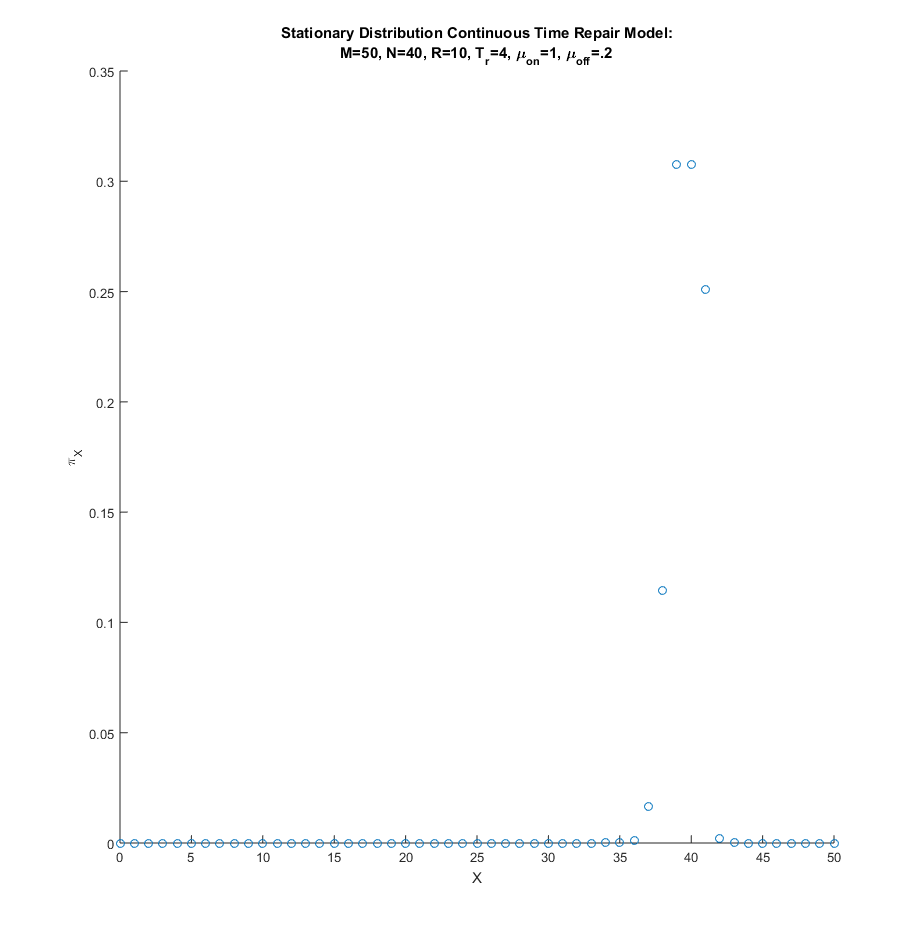
\includegraphics[width=400pt,height=400pt,keepaspectratio]{RepairModelStationaryDist1.png}
  \caption{This stationary distribution gives evidence that the factory is operating near optimally, with a low probability to be working below capacity and a high probability to be operating at full capacity. Further, depending on the fragility of machines a set up like this allows a high probability to have 1 or 2 relief machines}
\end{figure}
\begin{figure}
\centering
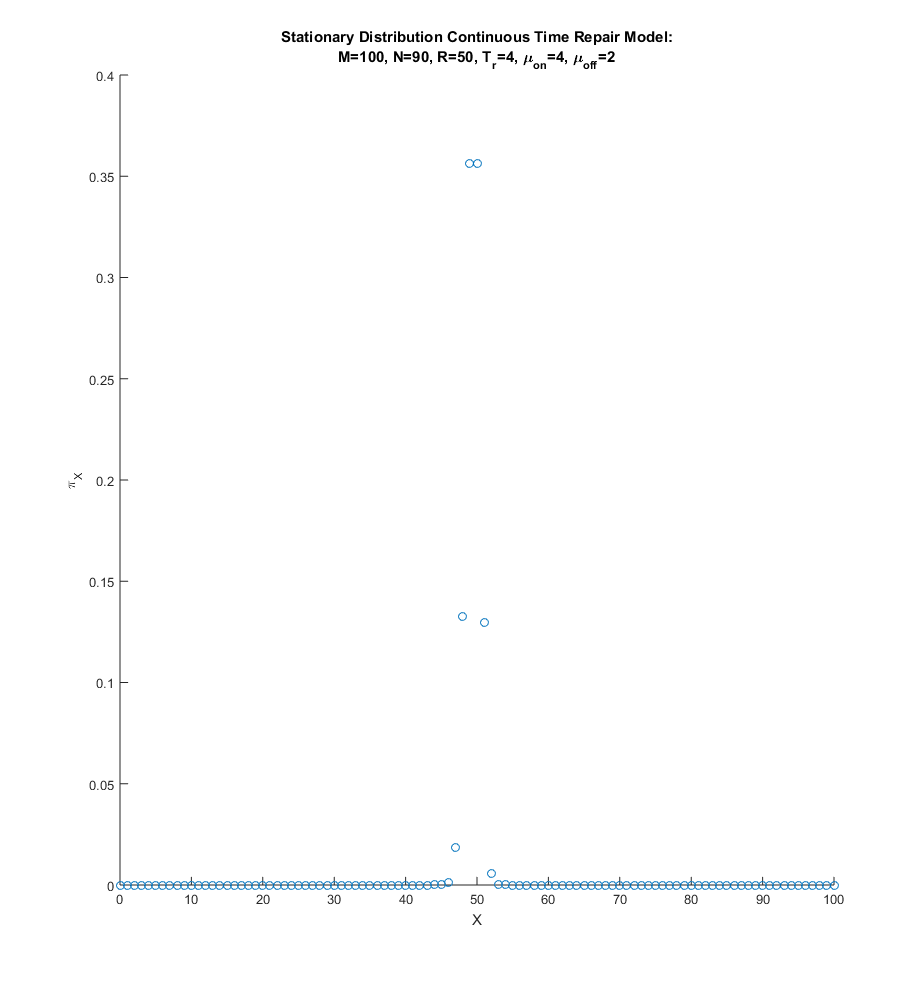
\includegraphics[width=400pt,height=400pt,keepaspectratio]{RepairModelStationaryDist2.png}
\caption{This stationary distribution gives evidence that the factory in question is operating at about half capacity most of the time. This may be due to having too few back up machines or machines that break too quickly to be repaired in time.}
\end{figure}
\begin{figure}
\centering
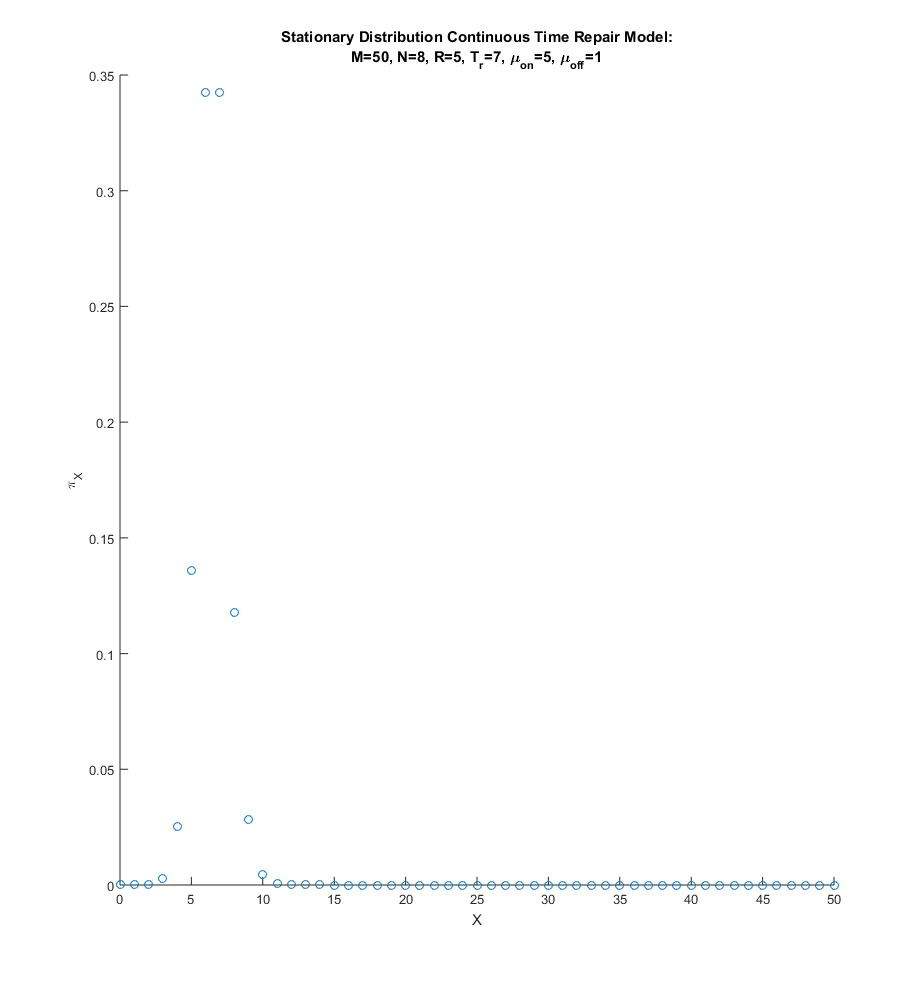
\includegraphics[width=400pt,height=400pt,keepaspectratio]{repairModelStationaryDist3.png}
\caption{This stationary distribution characterizes the limiting behavior of an assembly line working at near full capacity. There are an extremely large amount of machines in storage, but it is clear that most of these are run through quite quickly before the assembly line begins running inefficiently, likely due to a combination of the limits of the repair shop and the high failure rate of working machines.}
\end{figure}
\begin{figure}
\centering
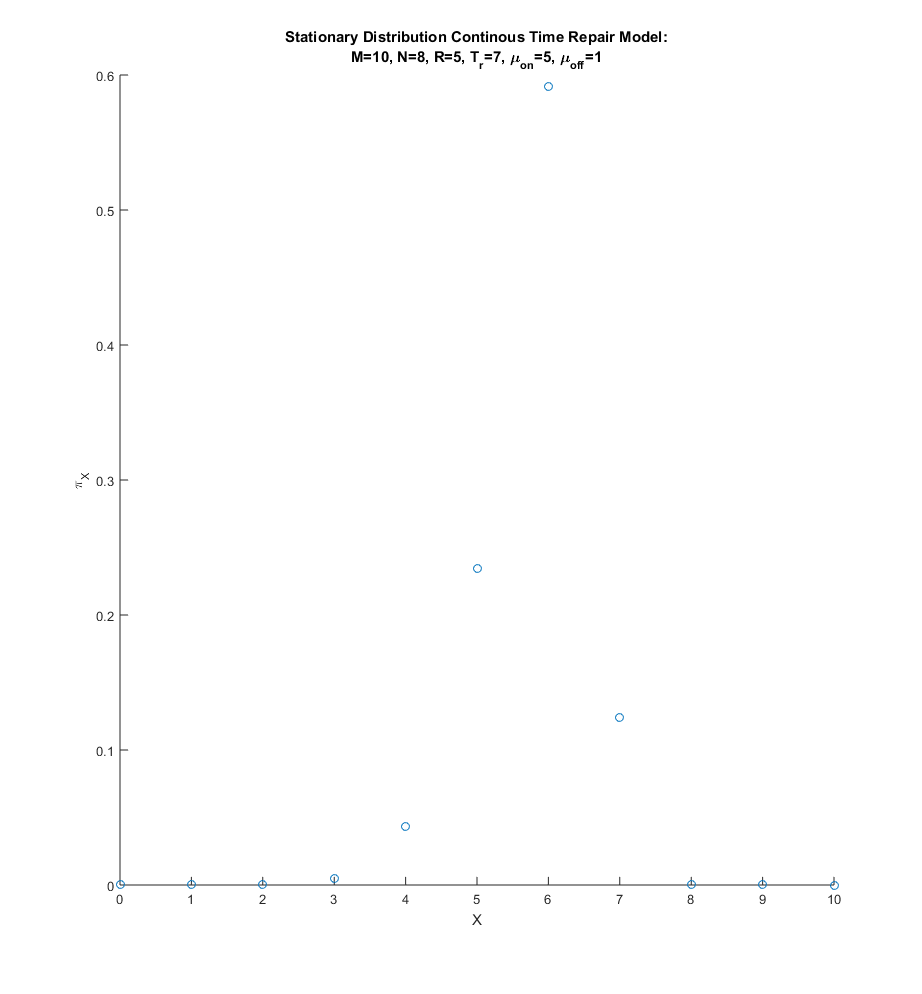
\includegraphics[width=400pt,height=400pt,keepaspectratio]{repairModelStationaryDist4.png}
\caption{This plot is a slight variation of the previous scenario. This realization shows that the assembly line can work at near optimal capacity with 1/5 of the back-up machines given the same parameters. Thus the limit on the assembly lines' productivity is clearly an issue with repairs or failure rate, suggesting a more reliable machine type is needed, or a better repair shop should be contracted.}
\end{figure}


    \end{subsection}
    \pagebreak
    \begin{subsection}{Extinction of Population with/without Finite Carrying Capacity}
    In this subsection, we consider an asexual population in an environment with limited resources, so that there is a maximum population size $K$. We will examine the continuous-time Markov chain model for the dynamics of the population through a birth-and-death process, with aggregate birth rate $\lambda i(1-i/K)$ and aggregate death rate $\mu i$ when the population has size $i$, where $\lambda$ and $\mu$ are the natural per capita birth and death rates of the population in the absence of competition for resources.\\

    Suppose the population starts with a single individual. For both the case of finite and infinite carrying capacity $K$, we calculate:\\
    \begin{enumerate}
        \item the probability that the population will eventually become extinct,
        \item The expected time until the population becomes extinct.
    \end{enumerate}
    Solution:\\

    We use the results from Karlin and Taylor 4.7 Theorem 7.1, which gives the extinction probability and mean time to extinction as follows for the case with an infinite carrying capacity. The probability of absorption into state 0 (death) from the initial state 1 is
    $$\left\{\begin{array}{cc}\frac{\sum_{i=1}^\infty\left(\prod_{j=1}^i \mu_j/ \lambda_j\right)}{1+\sum_{i=1}^\infty\left(\prod_{j=1}^i\mu_j/ \lambda_j\right)}& \text{ if }\sum_{i=1}^\infty\left(\prod_{j=1}^i \mu_j/\lambda_j\right) < \infty,\\
    \\
    1&\text{ if }\sum_{i=1}^\infty\left(\prod_{j=1}^i \mu_j/\lambda_j\right)=\infty\end{array}\right..$$
    The mean time to absorption is
    $$\left\{\begin{array}{cc}\infty &\text{ if }\sum_{i=1}^\infty\rho=\infty,\\
    \sum_{i=1}^\infty\rho_i& \text{ if }\sum_{i=1}^\infty \rho_i<\infty,\end{array}\right.$$
    where
    $$\rho_i=\frac{\lambda_1\lambda_2 \cdots \lambda_{i-1}}{\mu_1\mu_2\cdots\mu_i}.$$
    Then to find the $\lambda_i$ we must limit the given per capita birth rates as $K\to\infty$:
    $$\lim_{K\to\infty}\lambda i(1-i/K)=\lambda i.$$
    Now we inspect the sum in the probability of absorption into the extinction state by first looking at the sum $\sum_{i=1}^\infty\left(\prod_{j=1}^i \mu_j/\lambda_j\right)$. It is clear to see that the product inside of the sum can be rewritten
    $$\prod_{j=1}^i\frac{\mu_j}{\lambda_j}=\prod_{j=1}^i\frac{\mu j}{\lambda j}=\prod_{j=1}^i\frac{\mu}{\lambda}=\left(\frac{\mu}{\lambda}\right)^i.$$
    Then the sum we are looking at is a geometric sum sans the zeroth term (if $\lambda>\mu$):
    $$\sum_{i=1}^\infty\left(\prod_{j=1}^i \mu_j/\lambda_j\right)=\sum_{i=1}^\infty\left(\frac{\mu}{\lambda}\right)^i.$$
    Clearly, then, if $\mu\geq\lambda$ the sum is infinite and the probability of absorption into state 0 is 1. However, if $\lambda<\mu$ the sum is finite:
    $$\sum_{i=1}^\infty\left(\prod_{j=1}^i \mu_j/\lambda_j\right)=\sum_{i=1}^\infty\left(\frac{\mu}{\lambda}\right)=\frac{1}{1-\mu/\lambda}-1=\frac{\mu}{\lambda-\mu}.$$
    Therefore the absorption probability is
    $$\frac{\sum_{i=1}^\infty\left(\prod_{j=1}^i \mu_j/\lambda_j\right)}{1+\sum_{i=1}^\infty\left(\prod_{j=1}^i\mu_j/\lambda_j\right)}=\frac{\frac{\mu}{\lambda-\mu}}{1+\frac{\mu}{\lambda-\mu}}=\frac{\mu}{\lambda}.$$
    Thus for the infinite carrying capacity case of the linear birth and death process given the per capita birth and death rates, the extinction probability beginning with one individual is
    $$\left\{\begin{array}{cc}\frac{\mu}{\lambda} & \text{ if }\mu<\lambda\\1&\text{ if }\mu\geq\lambda\end{array}\right..$$
    Now we shift our attention to the mean time to absorption in the infinite carrying capacity case. We begin by defining $\rho_i$ given transition rates $\lambda_i=\lambda i$ and $\mu_i=\mu i$.
    $$\rho_i=\frac{\lambda_1\lambda_2\dots\lambda_{i-1}}{\mu_1\mu_2\dots\mu_i}=\frac{\lambda(2\lambda)(3\lambda)\dots(i-1)\lambda}{\mu(2\mu)(3\mu)\dots\mu(i-1)(i \mu)}=\frac{\lambda^{i-1}}{i\mu^i}=\left(\frac{\lambda}{\mu}\right)^i\frac{1}{\lambda i}$$
    Then the sum over the $\rho_i$s becomes
    $$sum_{i=1}^\infty\rho_i=\frac{1}{\lambda}\sum_{i=1}^\infty\left(\frac{\lambda}{\mu}\right)^i\frac{1}{i}.$$
    We then use the ratio test to find a relationship between $\lambda$ and $\mu$ such that the sum converges.
    $$\lim_{i\to\infty}\left|\left(\frac{\lambda}{\mu}\right)^{i+1}\frac{1}{i+1}\left(\frac{\mu}{\lambda}\right)^i i\right|=\left|\frac{\lambda}{\mu}\right|.$$
    Then since $\lambda,\mu\geq 0$ we have
    $$0\leq \frac{\lambda}{\mu}<1$$
    which gives
    $$0\leq\lambda<\mu.$$
    We need not check $\lambda=0$ as this result obviously will give a finite sum. In this case, the mean absorption time will be $1/\mu$. This is separate from the $\rho$ formulation as $\rho_i=0$. However, the mean absorption time should not be instantaneous, instead it must be the expected time that one person will die - $1/\mu$. We then check the case where $\lambda=\mu$. Substituting $\lambda=\mu$ into the sum formulated above gives
    $$\sum_{i=1}^\infty \frac{1}{\mu i}$$
    a harmonic series. Thus the mean time to absorption in the case where the per capita birth and death rates are equal is infinite. This is extremely interesting as the absorption probability here is 1. Then the ratio test tells us that the sum converges for $0\leq\lambda<\mu$. Then the mean time to absorption in the birth death process with infinite carrying capacity is
    $$\left\{\begin{array}{cc}\infty &\text{ if }\lambda\geq\mu\\ \frac{-1}{\lambda}\ln{\frac{\mu-\lambda}{\mu}}& \text{ if }0\leq \lambda<\mu\end{array}\right..$$

    In the case of the finite carrying capacity, we have an irreducible Markov chain with absorption probability 1. Using the birth rate for the finite carrying capacity as defined above, we can clearly see that if we use the same formulation as above but with upper bounds on the sums equal to $K$ we get an infinite-valued sum, due to $\lambda_K=0$. Thus we only need to check the mean absorption time. We then begin by defining $\rho$.
    $$\rho_i=\frac{\lambda(1-1/K)\lambda(1-2/K)\cdots\lambda(1-(i-1)/K)}{\mu(2\mu)\cdots(i\mu)}$$
    $$\rho_i=\left(\frac{\lambda}{\mu}\right)^i\frac{K}{\lambda K^{i} i!}\prod_{j=1}^{i-1}(K-j)$$
    Then summing over the $\rho$ gives
    $$\sum_{i=1}^K\rho_i=\sum_{i=1}^K\left(\frac{\lambda}{\mu}\right)^i\frac{K}{\lambda K^{i} i!}\prod_{j=1}^{i-1}(K-j)=\frac{1}{\lambda}\left[\left(\frac{K\mu+\lambda}{K\mu}\right)^K-1\right].$$
    Thus the only cases where we have issues with convergence using this formula are at $\mu=0$ and $\lambda=0$. At $\mu=0$, clearly absorption cannot happen and thus the developed formula gives a reasonable mean absorption time of infinity. At $\lambda=0$ we get a mean absorption time of $\frac{1}{\mu}$ given by limiting $\lambda\to 0$ in the condensed form of the sum, which is sensible, and equivalent to what we have in the infinite carrying capacity case.\\

    Lastly, as we limit $K$ to zero, the absorption probability must change to what we have developed in the beginning of this subsection, as we are simply changing the limit of the sum. However, we do find a strange result when we limit $K$ to infinity in the mean time to absorption formula.
    $$\lim_{K\to\infty}\frac{1}{\lambda}\left[\left(\frac{K\mu+\lambda}{K\mu}\right)^K-1\right]=\frac{e^{\lambda/\mu}-1}{\lambda}$$
    which is in contrast to the expression we found before:
    $$-\frac{1}{\lambda}\ln{\frac{\mu-\lambda}{\mu}}.$$
    Strangely, the new formula allows for calculation of mean absorption time for any values of $\lambda$ and $\mu$ with $\mu\neq 0$, whereas the first formula only works for the bounds listed above.

    \end{subsection}
    \begin{subsection}{Age Distribution in Pure Birth Process}
    We consider a rapidly growing asexual population with constant per capita birth rate, negligible death rate, and negligible competition for resources. In addition, we assume that the population starts with the introduction of a single newly created individual.\\
     To calculate the probability distribution for the size of the population after a time $t$, we solve the forward Kolmogorov equation using the transition rate matrix defined implicitly by
        $$A_{i,i}=-\lambda$$
        $$A_{i,i+1}=\lambda,$$
        where $\lambda$ is the per capita birth rate. This results in a system of differential equations that can be solved easily.
        $$\phi'_1(t)=-\lambda\phi_1(t)\implies \phi_1(t)=\lambda e^{-\lambda t}$$
        since the probability to produce an offspring in this case must be exponentially distributed.
        Then the solution to the second equation follows:
        $$\phi'_2=\lambda\phi_1-\lambda\phi_2\implies \phi_2'+\lambda\phi_2=\lambda^2 e^{-\lambda t}$$
        we use the method of integrating factors with $\mu=e^{\lambda t}$ to get
        $$(\phi_2e^{\lambda t})'=\lambda^2 t+C\implies \phi_2=\lambda^2 te^{-\lambda t}$$
        as the initial conditions require $C=0$.\\
        The process to solve the rest of the equations is the same, with each constant of integration being 0. Thus we get the solution for each $\phi_j$:
        $$\phi_j(t)=\frac{\lambda(\lambda t)^{j-1}}{(j-1)!}e^{-\lambda t}.$$
        Then we know the probability that there are $j$ individuals at time $t$ to be the $\phi_j(t)$. Then, looking at the form for arbitrary $\phi_j(t)$ we see that the probability distribution for the size of the population after time $t$ is a gamma distribution with mean $\frac{j}{\lambda}$.
        \end{subsection}
   % \begin{subsection}{Population Model with Immigration}
%    Here we want to model a population with per capita birth rate $\lambda$, per capita death rate $\mu$, and an aggregate immigration rate of $\nu$. We suppose that the dynamics of the population size can be modeled by a continuous-time Markov chain with the usual birth-and-death model, modified to account for immigration. We will derive criteria on $\lambda$, $\mu$, and $\nu$ for the following to have probability 1 to be true:
%    \begin{enumerate}
%        \item The population will always remain bounded by some fixed value.
%        \item The population size is guaranteed to eventually never fall below 1000.
%        \item The population will repeatedly be reduced to zero size.
%        \item The expected time is finite between the first and the second time the population falls to zero size.
%    \end{enumerate}
%    We begin by defining the birth and death parameters $\lambda_n$ and $\mu_n$;
%    $$\lambda_n=\lambda n+\nu$$
%    $$\mu_n=\mu n.$$
%    Thus the transition rate matrix can be defined as follows:
%    $$A_{i,i-1}=i \mu$$
%    $$A_{i,i+1}=i\lambda +\nu $$
%    $$A_{i,i}=-i(\mu+\lambda)-\nu.$$

    \begin{subsection}{Stochastic Chemistry}
    In this subsection we consider an enzyme-catalyzed irreversible chemical reaction:
    $$S+E\rightarrow^{k_1}C+E,\quad C+C\rightarrow^{k_2}P,$$
    where $S$ denotes a substrate molecule, $E$ an enzyme molecule, $C$ an intermediate complex molecule, and $P$ the product molecule. The rate constants $k_1$ and $k_2$ mean that the rates per volume of the two chemical reactions are, respectively, $k_1(N_S/V)(N_E/V)$ and $k_2(N_C/V)((N_C-1)/V)$, where the subscripted $N$ variables refer to the number of that type of molecule in the reaction chamber with volume $V$, in which we assume all variables are well-mixed. The factor $N_C-1$ in the second reaction rate expression arises from the fact a complex molecule must find another complex molecule to react with and there are $N_C-1$ complex molecules other than itself to pair with. We will further assume that the substrate is available in such great supply that we can neglect the change in $N_S$ due to the chemical reaction.\\

    We can formulate a variation of a continuous-time birth-death process Markov chain model to describe $N_C$ the number of intermediate complex molecules to describe the concentration density of the molecule, denoted $C$, using the relationship $N_C/V=C$. We denote the Markov chain to be $\{N_C(t)\}$ where $N_C$ is the number of molecules $C$ at time $t$. The state space of our model must be $\mathbb{Z}_{\geq 0}$ such that if the reaction runs to completion, there will be no $C$ molecules left and it allows for the number of $C$ molecules to grow infinitely if the first reaction is fast while the second is slow.\\

        The birth rate of the molecule $C$ is the reaction rate of the first reaction
        $$\lambda_i=\frac{k_1 N_SN_E}{V^2}.$$
        The birth rate is constant for all $i$, since we ignore the change in $N_S$. The death rate, however, requires a variation from the usual death process because two molecules 'die' at once. We have
        $$\mu=\frac{k_2N_C(N_C-1)}{V^2}.$$
        However, $\mu$ is not constant over the state space, since the state space is the number of intermediate molecules. Thus we have
        $$\mu_i=\frac{k_2 i(i-1)}{V^2}.$$
        This allows us to define a transition rate matrix with entries
        $$A_{i,i+1}=\frac{k_1 N_SN_E}{V^2},$$
        $$A_{i,i-2}=\frac{k_2 i(i-1)}{V^2},$$
        $$A_{i,i}=-\left(\frac{k_2 i(i-1)}{V^2}+\frac{k_1 N_SN_E}{V^2}\right),$$
        $$A_{i,j}=0\quad \text{otherwise}.$$

        \end{subsection}
    \end{section}
    \begin{section}{Mathematical Problems}
    \begin{subsection}{Stationary Distributions for Continuous-Time and Embedded Discrete-Time Markov Chain}
    We suppose an irreducible continuous-time Markov chain with transition rate matrix $A$ has stationary distribution $\mathbf{\pi}$. We then consider the embedded discrete-time Markov chain defined by the successive states visited by the continuous-time Markov chain. We will describe precisely how the stationary distribution of this discrete-time Markov chain, denoted $\mathbf{\eta}$, is associated to $A$ and $\mathbf{\pi}$.\\

    We begin by defining the entries in $A$ and $P$, the probability transition rate matrix for the embedded discrete Markov chain. The entries of $A$ are the transition rates $a_{ij}$ where $a_{ii}=-\sum_{j\neq i}a_{ij}$. We can define the entries of $P$, $p_{ij}$ to be the normalized transition rates out of state $i$ with each $p_{ii}=0$. Therefore
    $$p_{ij}=\frac{a_{ij}}{a_{ii}}.$$
    To define a stationary distribution for a discrete-time Markov chain, $\mathbf{\eta}$ must satisfy
    $$\mathbf{\eta}=\mathbf{\eta}P.$$
    Similarly, $\mathbf{\pi}$ must satisfy
    $$0=\mathbf{\pi}A.$$
    Then, writing the $j$th inner product in each matrix-vector multiplication gives
    $$\pi_ja_{ii}=\sum_{i\neq j}\pi_i a_{ij}$$
    $$\eta_j=\sum_{i\in S}\eta_ip_{ij}.$$
    We can rewrite the first of the pair of equations using the relationship $a_{ij}=a_{ii}p_{ij}$ to get
    $$\pi_ja_{jj}=\sum_{i\in S}\pi_ia_{ii}p_{ij}.$$
    This gives the desired relationship
    $$C\pi_ja_{jj}=\eta_j,$$
    where $C$ is an appropriate normalizing constant.
    
    
    \end{subsection}
\end{section}
\pagebreak
\begin{section}{Numerical Simulation}
\begin{subsection}{Stochastic Epidemic Model}
In this section we develop a computer program to simulate the progress of an epidemic according to the stochastic SIR model discuessed in class. We assume that the probability distribution for the duration of the infectious period of the illness is gaussian with mean $\mu$ and variance $\sigma^2$. The mean $\mu$ can be interpreted as the average duration of the illness. The program allows the user to specify
\begin{itemize}
\item the initial susceptible population
\item the initial infected population
\item the rate at which the infection is communicated to susceptibles
\item the mean and variance of the recovery times.
\end{itemize}
The code for the program is as follows:
\begin{lstlisting}
function [timeMat,susceptMat,infectMat,recovMat]=stochasticEpidemicModel(S0,I0,lambda,meanIll,sDevIll,maxTime)
%This function simulates a continuous time stochastic epidemic model
%using the next-event update method.
%S0 and I0 are the initial populations of susceptible and infected
%individuals and N is the size of the total population
%lambda is the rate at which the infection is communicated to susceptibles
%we will choose a normal distribution with mean meanill and std. deviation
%sDevIll as the recovery time distribution.

I=I0;
S=S0;
N=S+I;
%Assign infection threshold for each susceptible individual which are
%exponentially distributed random variables with mean 1
phi=exprnd(1,[1,S0]);
%order phi
phi=sort(phi);

%Assign simulated Recovery Times to each susceptible and infected individual
T = meanIll + sDevIll.*randn(1,I0+S0);

%Simulation of the model
count=1;
time=0;
%Save initial state
timeMat(count,1)=time;
susceptMat(count,1)=S;
infectMat(count,1)=I;
recovMat(count,1)=N-S-I;
while I>0&&time<maxTime
    if I==0
        break
    end
    count=count+1;
    newTime=exprnd(1/lambda);
    b=min(I,numel(T));
    if newTime<min(T(1,1:b))
        %Calculate Infection Pressure
        sumPress=0;
        b=min(I,numel(T));
        %remove the elapsed time from the recovery times
        T(1,1:b)=T(1,1:b)-newTime*ones(1,b);
        for i=1:b
            sumPress=T(i)+sumPress;
        end
        infPress=(lambda*sumPress)/N;
        %Decide how many susceptibles get infected during the maximum infection
        %pressure
        sumPhi=0;
        i=1;
        while sumPhi<infPress&&phi(i)>0
            sumPhi=phi(i)+sumPhi;
            i=i+1;
            if i>numel(phi)
                break
            end
        end

        %Remove the newly infected person(s) from the infection threshold
        if i>S
            phi=0;
        else
            phi=phi(1,i:S);
        end
        %Increment I, S and time
        I=I+i-1;
        S=S-i+1;
        time=time+newTime;
        %Save the times that events happen, along with the population size at
        %those times
        timeMat(count,1)=time;
        susceptMat(count,1)=S;
        infectMat(count,1)=I;
        recovMat(count,1)=N-S-I;
    else
        %Let the soonest recovery happen, then restart the loop
        b=min(I,numel(T));
        time=time+min(T(1,b));
        m=numel(T);
        T(1,1:b)=T(1,1:b)-min(T(1,1:b))*ones(1,b);

        %Decrement I from the soonest recovery
        I=I-1;

        %Remove the infection from the infection times
        [~,j]=min(T(1,1:b));
        T=T([1:j-1,j+1:m]);
        %Save the times that events happen, along with the population size at
        %those times
        timeMat(count,1)=time;
        susceptMat(count,1)=S;
        infectMat(count,1)=I;
        recovMat(count,1)=N-S-I;
    end

end

%plot SIR classes over time
plot(timeMat,susceptMat,timeMat,infectMat,timeMat,recovMat)
legend('Susceptible','Infected', 'Recovered')
xlabel('Time')
ylabel('Population')
title('Stochastic Epidemic Model')

\end{lstlisting}
See two plots of this function attached. Each plot uses the same parameters, but shows that we can get both an endemic and nonendemic scenario solely from the different random variables in each iteration. The parameter values are in the title.\\
We also developed a histogram for the total number of people eventually infected by the disease. For interesting results, we chose a slightly different set of parameters than in the plotted scenario. We use the code below to plot the histogram for the total number of people eventually infected by the disease: 
\begin{lstlisting}
function iterateStochasticEpidemicModel(S0,I0,lambda,meanIll,sDevIll,maxTime)
for i=1:1000
    [timeMat,susceptMat,infectMat,recovMat]=stochasticEpidemicModel(S0,I0,lambda,meanIll,sDevIll,maxTime);

    n=numel(infectMat);
    m=numel(recovMat);
    everInfected(1,i)=recovMat(m)+infectMat(n);
end
histogram(everInfected)
\end{lstlisting}
See attached for the plot of the histogram.
\end{subsection}
\begin{figure}
\centering
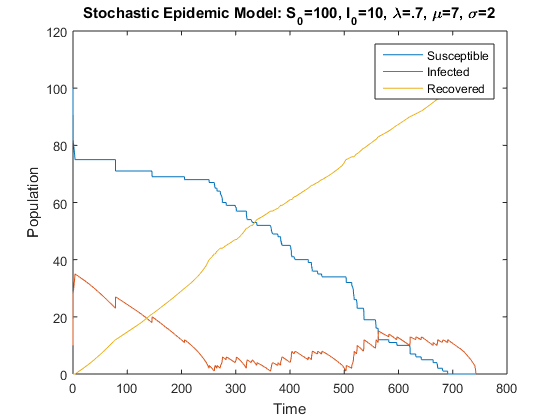
\includegraphics[width=400pt]{SIRModelEndemic}
\end{figure}
\begin{figure}
\centering
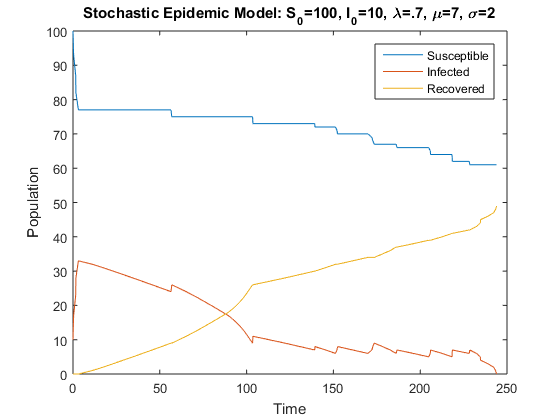
\includegraphics[width=400pt]{SIRModelLife}
\end{figure}
\end{section}

\end{document} 